\section{Wheel Brake System}
\label{sec:wbs}
To demonstrate the fault modeling capabilities of the Safety Annex we will use the Wheel Brake System (WBS) described in AIR6110~\cite{AIR6110}.  This system is a well-known example that has been used as a case study for safety analysis, formal verification, and contract based design~\cite{DBLP:conf/cav/BozzanoCPJKPRT15, 10.1007/978-3-319-11936-6-7, CAV2015:BoCiGrMa, Joshi05:SafeComp}. The preliminary work for the Safety Annex was based on a simple model of the WBS~\cite{Stewart17:IMBSA}. To demonstrate a more complex fault modeling process, we constructed a functionally and structurally equivalent AADL version of the more complex WBS NuSMV/xSAP models~\cite{DBLP:conf/cav/BozzanoCPJKPRT15}.    

\begin{figure}[htbp]
	\centering
	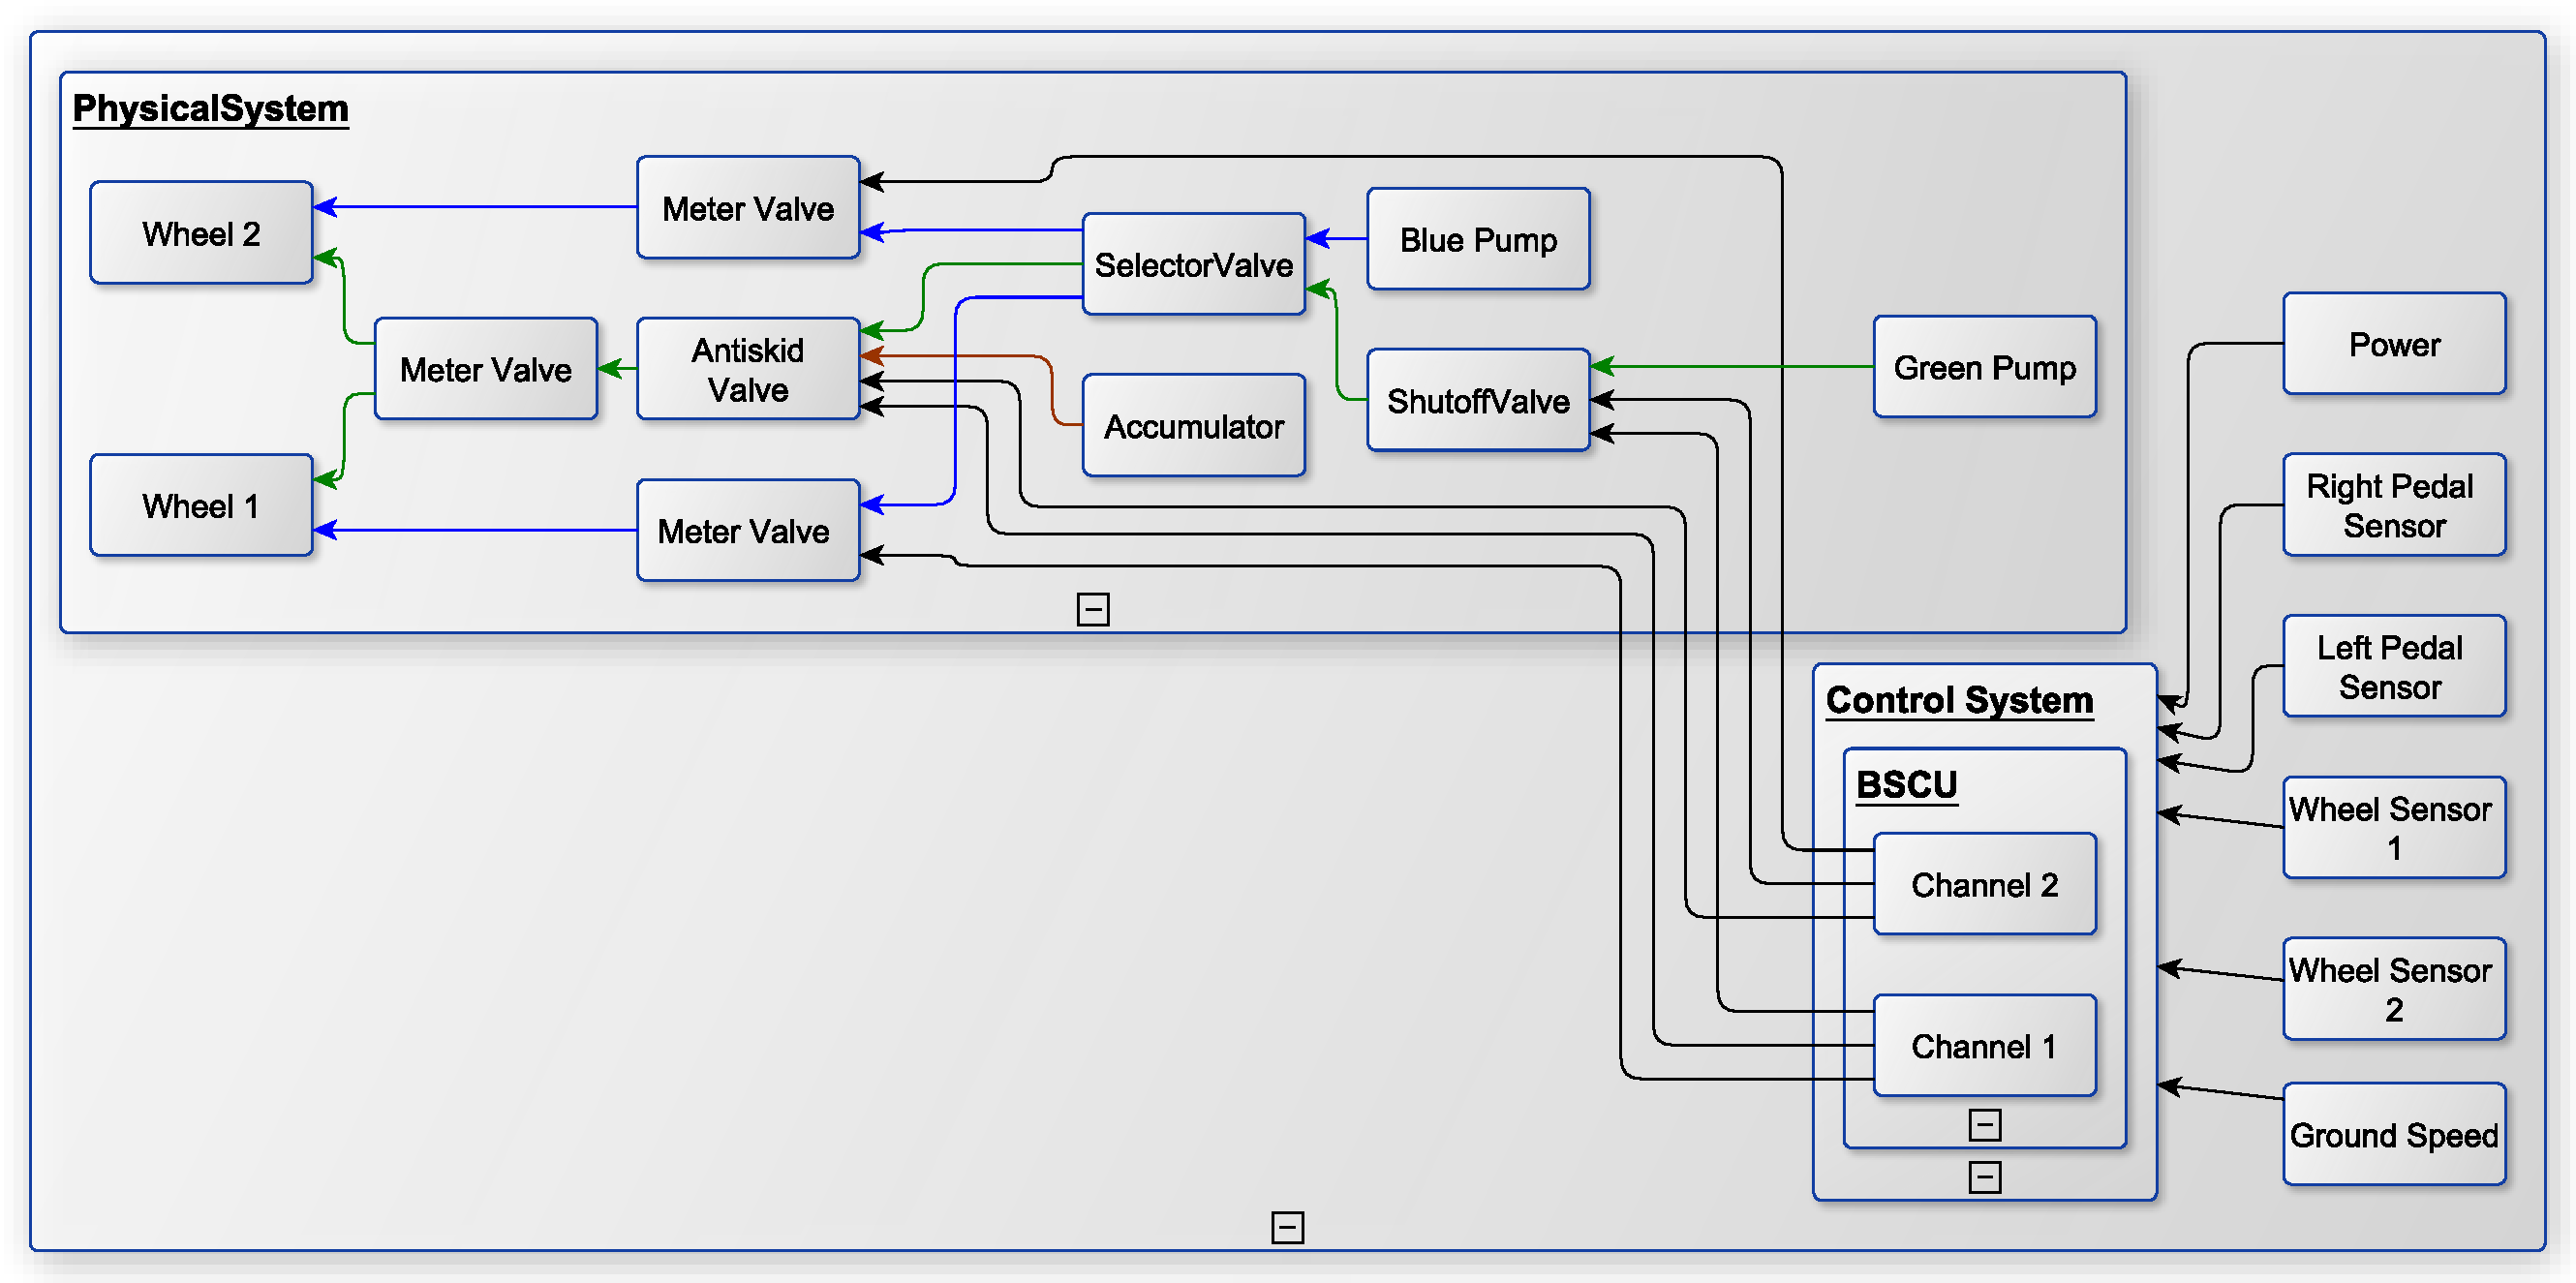
\includegraphics[trim=0 9 0 5,clip,width=\textwidth]{images/wbs_arch4_diagram.pdf}
	\caption{Simplified Two-wheel Wheel Brake System}
	\label{fig:wbs}
\end{figure} 

The WBS is composed of two main parts: the Line Replaceable Unit control system and the electro-mechanical physical system.
The control system electronically controls the physical system and contains a redundant
channel of the Braking System Control Unit (BSCU) in case a detectable fault occurs in the active channel.
 It also commands antiskid braking. % in case of skidding on the ground. 
 The physical system consists of the hydraulic circuits running from hydraulic pumps to wheel brakes as well as valves that control the hydraulic fluid flow. This system provides braking force to each of the eight wheels of the aircraft. The wheels are all mechanically braked in pairs (one pair per landing gear). For simplicity, Figure~\ref{fig:wbs} displays only two of the eight wheels. 

There are three operating modes in the WBS model:

\begin{itemize}
	\renewcommand{\labelitemi}{\textbullet}
	\item In \textit{normal} mode, the system is composed of a \textit{green} hydraulic pump and one meter valve per each of the eight wheels. Each of the meter valves are controlled through electronic commands coming from the active channel of the BSCU. These signals provide braking and antiskid commands for each wheel. The braking command is determined through a sensor on the pedal and the antiskid command is determined by the \textit{Wheel Sensors}. 
	\item In \textit{alternate} mode, the system is composed of a \textit{blue} hydraulic pump, four meter valves, and four antiskid shutoff valves, one for each landing gear. The meter valves are mechanically commanded through the pilot pedal corresponding to each landing gear. If the selector detects lack of pressure in the green circuit, it switches to the blue circuit. 
	\item In \textit{emergency} mode, the system mode is entered if the \textit{blue} hydraulic pump fails. The accumulator pump has a reserve of pressurized hydraulic fluid and will supply this to the blue circuit in emergency mode. 
\end{itemize}

The WBS architecture model in AADL contains 30 different kinds of components, 169 component instances, and a model depth of 5 hierarchical levels. 

The behavioral model is encoded using the AGREE annex and the behavior is based on descriptions found in AIR6110. The top level system properties are given by the requirements and safety objectives in AIR6110. All of the subcomponent contracts support these system safety objectives through the use of assumptions on component input and guarantees on the output. The WBS behavioral model in AGREE annex includes one top-level assumption and  11 top-level system properties, with 113 guarantees allocated to subsystems.  

An example system safety property is to ensure that there is no inadvertent braking of any of the wheels. This is based on a failure condition described in AIR6110 is \textit{Inadvertent wheel braking on one wheel during takeoff shall be less than 1E-9 per takeoff}. 
Inadvertent braking means that braking force is applied at the wheel but the pilot has not pressed the brake pedal.  In addition, the inadvertent braking requires that power and hydraulic pressure are both present, the plane is not stopped, and the wheel is rolling (not skidding). The property is stated in AGREE such that inadvertent braking does \textit{not} occur, as shown in Figure \ref{fig:inadvertent_braking}. 

\begin{figure}[htbp]
	%\vspace{-0.2in}
	\begin{center}
		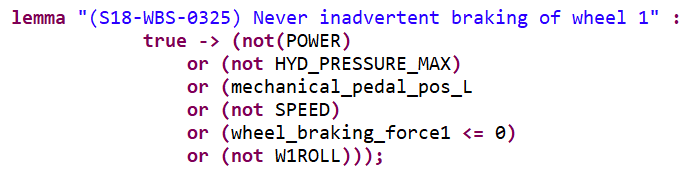
\includegraphics[width=.7\textwidth]{images/inadvertent_braking.png}
	\end{center}
	\vspace{-0.3in}
	\caption{AGREE Contract for Top Level Property: Inadvertent Braking}
	\label{fig:inadvertent_braking}
	%\vspace{-0.2in}
\end{figure}

\subsection{Nominal Model Analysis}
Before performing fault analysis, users should first check that the safety properties are satisfied by the nominal design model. This analysis can be performed monolithically or compositionally in AGREE. Using monolithic analysis, the contracts at the lower levels of the architecture are flattened and used in the proof of the top level safety properties of the system. Compositional analysis, on the other hand, will perform the proof layer by layer top down, essentially breaking the larger proof into subsets of smaller problems. For a more comprehensive description of these types of proofs and analyses, see additional publications related to AGREE \cite{cofer2012compositional,QFCS15:backes} 

The WBS has a total of 13 safety properties at the top level that are supported by subcomponent assumptions and guarantees. These are shown in Table \ref{tab:safetyProperties}. Given that there are 8 wheels, contract S18-WBS-0325-wheelX is repeated 8 times, one for each wheel. The behavioral model in total consists of 36 assumptions and 246 supporting guarantees.
\begin{center}
\begin{table}[htbp]
\begin{tabular}{@{}ll}
\toprule
\textbf{S18-WBS-R-0321} \\Loss of all wheel braking during landing or RTO shall be less than $5.0 \times 10^{-7}$ per flight.                                    \\ \midrule 
\textbf{S18-WBS-R/L-0322}  \\ Asymmetrical loss of wheel braking (Left/Right) shall be less than $5.0 \times 10^{-7}$ per flight. \\ \midrule
\textbf{S18-WBS-0323} \\ Never inadvertent braking with all wheels locked shall be less than $1.0 \times 10^{-9}$ per takeoff.                                                                                                                                                                                                               \\ \midrule
\textbf{S18-WBS-0324}  \\ Never inadvertent braking with all wheels shall be less than $1.0 \times 10^{-9}$ per takeoff.                                                                                                            \\ \midrule
\textbf{S18-WBS-0325-wheelX} \\ Never inadvertent braking of wheel X shall be less than $1.0 \times 10^{-9}$ per takeoff.                                                                                                           .                                                                                                                 \\ \bottomrule
\end{tabular}
\caption{Safety Properties of WBS}
\label{tab:safetyProperties}
\end{table} 
\end{center} 

\subsection{Fault Model Analysis}
There are two main options for fault model analysis using the Safety Annex. The first option injects faulty behavior allowed by faulty hypothesis into the AGREE model and returns this model to JKind for analysis. This allows for the activity of faults within the model and traceability information provides a way for users to view a counterexample to a violated contract in the presence of faults. The second option is used to generate minimal cut sets for the model. The model is annotated with fault activation that are constrained to false as well as intermediate level guarantees as model elements for consideration for the all Minimal Inductive Validity Cores (All-MIVCs)
algorithm. The All-MIVCs traces the minimal set of model elements used to produce minimal cut sets. This subsection presents these options and discusses the analytical results obtained. 

\subsubsection{Verification in the Presence of Faults: Max N Analysis}
Using a max number of faults for the hypothesis, the user can constrain the number of simultaneously active faults in the model. The faults are added to the AGREE model for the verification. Given the constraint on the number of possible simultaneously active faults, the model checker attempts to prove the top level properties given these constraints. If this cannot be done, the counterexample provided will show which of the faults (N or less) are active and which contracts are violated. 

The user can choose to perform either compositional or monolithic analysis using a max N fault hypothesis. In compositional analysis, the analysis proceeds in a top down fashion. To prove the top level properties, the properties in the layer directly beneath the top level are used to perform the proof. The analysis proceeds in this manner. Users constrain the maximum number of faults within each layer of the model by specifying the maximum fault hypothesis statement to that layer. If any lower level property failed due to activation of faults, the property verification at the higher level can no longer be trusted because the higher level properties were proved based on the assumption that the direct sub-level contracts are valid. This form of analysis is helpful to see weaknesses in a given layer of the system. 

In monolithic analysis the layers of the model are flattened, which allows a direct correspondence between all faults in the model and their effects on the top level properties. As with compositional analysis, a counterexample shows these N or less active faults. 

\subsubsection{Verification in the Presence of Faults: Probabilistic Analysis} 
Given a probabilistic fault hypothesis, this corresponds to performing analysis with the combinations of faults whose occurrence probability is less than the probability threshold. This is done by inserting assertions that allow those combinations in the Lustre code. If the model checker proves that the safety properties can be violated with any of those combinations, one of such combination will be shown in the counterexample. 

Probabilistic analysis done in this way must utilize the monolithic AGREE option. For compositional probabilistic analysis, see Section~\ref{sec:prob_generate}.

To perform this analysis, it is assumed that the non-hardware faults occur independently and possible combinations of faults are computed and passed to the Lustre model to be checked by the model checker. As seen in Algorithm 1, the computation first removes all faults from consideration that are too unlikely given the probability threshold. The remaining faults are arranged in a priority queue $\mathcal{Q}$ from high to low. Assuming independence in the set of faults, we take a fault with highest probability from the queue (step 5) and attempt to combine the remainder of the faults in $\mathcal{R}$ (step 7). If this combination is lower than the threshold (step 8), then we do not take into consideration this set of faults and instead remove the tail of the remaining faults in $\mathcal{R}$. 
 
\begin{algorithm}[H]
	% \KwData{this text}
	% \KwResult{how to write algorithm with \LaTeX2e }
	$\mathcal{F} = \{\}$ : fault combinations above threshold \;
	$\mathcal{Q}$ : faults, $q_i$, arranged with probability high to low \;
	$\mathcal{R} = \mathcal{Q}$ , with $r \in \mathcal{R}$\;
	\While{$\mathcal{Q} \neq \{\} \land \mathcal{R} \neq \{\}$ }{
		$q =$ removeTopElement($\mathcal{Q}$) \;
		\For{$i=0:|\mathcal{R}|$}{
			$prob = q \times r_i$ \;
			\eIf{prob $<$ threshold}{
				removeTail($\mathcal{R}, j=i:|\mathcal{R}|$)\;
			}{
				add($\{q, r_i\}, \mathcal{Q}$)\;
				add($\{q, r_i\}, \mathcal{F}$)\;
			} % end if else
		} % end for
	} % end while
	\caption{Monolithic Probability Analysis}
	\label{alg:prob_monolithic}
\end{algorithm}
In this calculation, we assume independence among the faults, but in the Safety Annex it is possible to define dependence between faults using a fault propagation statement. After fault combinations are computed using Algorithm~\ref{alg:prob_monolithic}, the triggered dependent HW faults are added to the combination as appropriate. The dependencies are implemented in the \textit{Verify in the Presence of Faults} options for analysis, but not yet implemented in the \textit{Generate Minimal Cut Sets} analysis options.

\subsubsection{Generate Minimal Cut Sets: Max N Analysis}
\label{sec:maxN_generate}
As described in Chapter~\ref{chap:mcsGen}, the generation of MinCutSets uses the All-MIVCs algorithm to provide a full enumeration of all minimal set of model elements necessary for the proof of each top-level safety property in the model, and then transforms all MIVCs into all minimal cut sets. In Max N analysis, the minimal cut sets are pruned to include only those with at cardinality less or equal to the max N number specified in the fault hypothesis and displayed to the user.

Generate MinCutSet analysis was performed on the Wheel Brake System and results are shown in Table~\ref{tab:wbs_maxN_results}. Notice in Table~\ref{tab:wbs_maxN_results}, the label across the top row refers to the cardinality (C) and the corresponding column shows how many cut sets are generated of that cardinality. When the analysis is run, the user specifies the value N. This gives cut sets of cardinality \textit{less than or equal to} N. (For the full text of the properties, see Table~\ref{tab:safetyProperties}.)

\begin{center}
\begin{table}[htbp]
    \begin{tabular}{ | l | l | l | l | l | l | l | l |}
    \hline
    \textbf{Property} & $\bm{c = 1}$ & $\bm{c = 2}$ & $\bm{c = 3}$ & $\bm{c = 4}$ 
		& $\bm{c = 5}$ & $\bm{c = 6}$ & $\bm{c = 7+}$  \\ \hline \hline
    R-0321 & 6 & 0 & 0 & 1& 144&7776 &- \\ \hline
    R-0322 & 32 & 0 & 0 &0 &0 &0 &- \\ \hline
    L-0322 & 32 & 0 & 0 &0 &0 &0 &- \\ \hline
    0323 & 90 & 0 & 0 &0 &0 &0 &- \\ \hline
    0324 & 8 & 3,401 & 6,800 &66,472 & 435,358&1,892,832 &- \\ \hline
    0325-WX & 20 & 0 & 0 &0 &0 & 0&- \\ \hline
    \end{tabular}
    \caption{WBS MinCutSet Analysis Results for Cardinality $c$}
    \label{tab:wbs_maxN_results}
\end{table}
\end{center}

Due to the increasing number of possible fault combinations at $N=6$, the computational time increases quickly. The WBS analysis was only run to $N=6$ for this reason. 

\subsubsection{Generate Minimal Cut Sets: Probabilistic Analysis}
\label{sec:prob_generate}
Both probabilistic analysis and max N analysis use the same minimal cut set generation algorithm, except that in probabilistic analysis, the minimal cut sets are pruned to include only those fault combinations whose probability of simultaneous occurrence exceed the given threshold in the probability hypothesis. Note that with probablistic hypothesis, \textit{Verify in the Presence of Faults} is performed using only monolithic analysis, but generating minimal cut sets is performed using compositional analysis.


The probabilistic analysis for the WBS was given a top level threshold of $1.0 \times 10^{-9}$ as stated in AIR6110. The faults associated with various components were all given probability of occurrence compatible with the discussion in this same document. 

As shown in Table~\ref{tab:wbs_prob_results}, the number of allowable combinations drops considerably when given probabilistic threshold as compared to just fault combinations of certain cardinalities. For example, one contract (inadvertent wheel braking of all wheels) had over a million minimal cut sets produced when looking at it in terms of max N analysis, but after taking probabilities into account, it is seen that only one combination of faults can violate this property. (For the full text of the properties, see Table~\ref{tab:safetyProperties}.)

\begin{center}
\begin{table}[htbp]
    \begin{tabular}{ | l | l | l | l | l | l | l | l | l |}
    \hline
    \textbf{Property} & $\bm{c = 1}$ & $\bm{c = 2}$ & $\bm{c = 3}$ & $\bm{c = 4}$ 
		& $\bm{c = 5}$ & $\bm{c = 6}$ & $\bm{c = 7}$ & $\bm{c = 8}$  \\ \hline \hline
    R-0321 & 0 & 0 & 0 & 0 & 0 & 0 & 0 & 0 \\ \hline
    R-0322 & 32 & 0 & 0 &0 &0 &0 &0& 0  \\ \hline
    L-0322 & 32 & 0 & 0 & 0 & 0 & 0 & 0 & 0  \\ \hline
    0323 & 90 & 0 & 0 & 0 & 0 & 0 & 0 & 0  \\ \hline
    0324 & 0 & 1 & 0 & 0 & 0 & 0 & 0 & 0  \\ \hline
    0325-WX & 20 & 0 & 0 &0 &0 & 0 & 0 & 0  \\ \hline
    \end{tabular}
    \caption{WBS MinCutSet Results for Probabilistic Analysis}
    \label{tab:wbs_prob_results}
\end{table}
\end{center}

\subsubsection{Results from Generate Minimal Cut Sets}
Results from Generate Minimal Cut Sets analysis can be represented in one of the following forms.
\begin{enumerate}
\item The minimal cut sets can be presented in text form with the total number per property, cardinality of each, and description strings showing the property and fault information. A sample of this output is shown in Figure~\ref{fig:detailedMCS}. 
\begin{figure}[htbp]
	\hspace*{-2cm}
	\vspace{-0.1in} 
	\begin{center}
		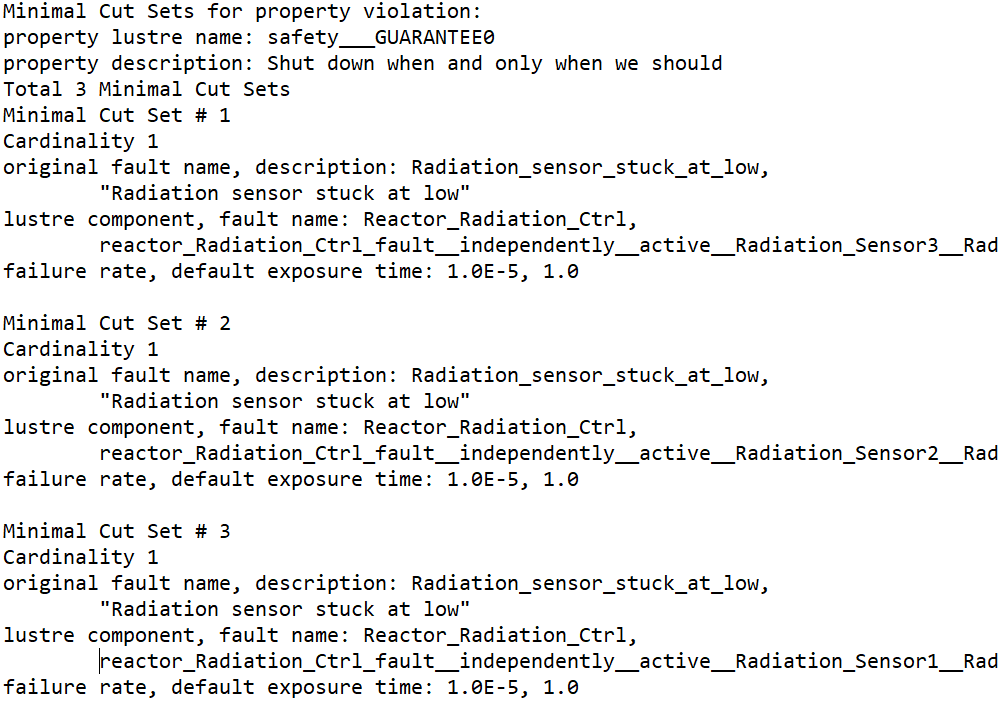
\includegraphics[scale=0.7]{images/detailedMCS.png}
	\caption{Detailed Output of MinCutSets}
		\label{fig:detailedMCS}
	\end{center}
\end{figure}

\item The minimal cut set information can be presented in tally form. This does not contain the fault information in detail, but instead gives only the tally of cut sets per property. This is useful in large models with many cut sets as it reduces the size of the text file. An example of this output type is seen in Figure~\ref{fig:tallyMCS}.
\begin{figure}[htbp]
	\hspace*{-2cm}
	\vspace{-0.1in} 
	\begin{center}
		\includegraphics[scale=0.7]{images/TallyMCS.png}
	\caption{Tally Output of MinCutSets}
		\label{fig:tallyMCS}
	\end{center}
\end{figure}

\item The tool can also generate fault tree and minimal cut set information formatted as input to the SOTERIA tool~\cite{manolios2019model} to produce hierarchical fault trees that are consistent with the system architecture/component verification layers, or flat fault trees consist of minimal cut sets only, both in graphical form. A sample graphical fault tree output from the SOTERIA tool is shown in Figure~\ref{fig:soteriaFT}. The SOTERIA tool is also able to compute the probabilities for the top level event from a given fault tree. However, based on experience with the WBS example, our tool was a more scalable solution as it produces minimal cut sets for more complex systems, also in shorter amount of time. The text format of the minimal cut sets seemed anectodally easier to read than the graphical format for larger systems.  
\begin{comment}
\begin{figure}[htbp]
	\hspace*{-2cm}
	\vspace{-0.1in} 
	\begin{center}
		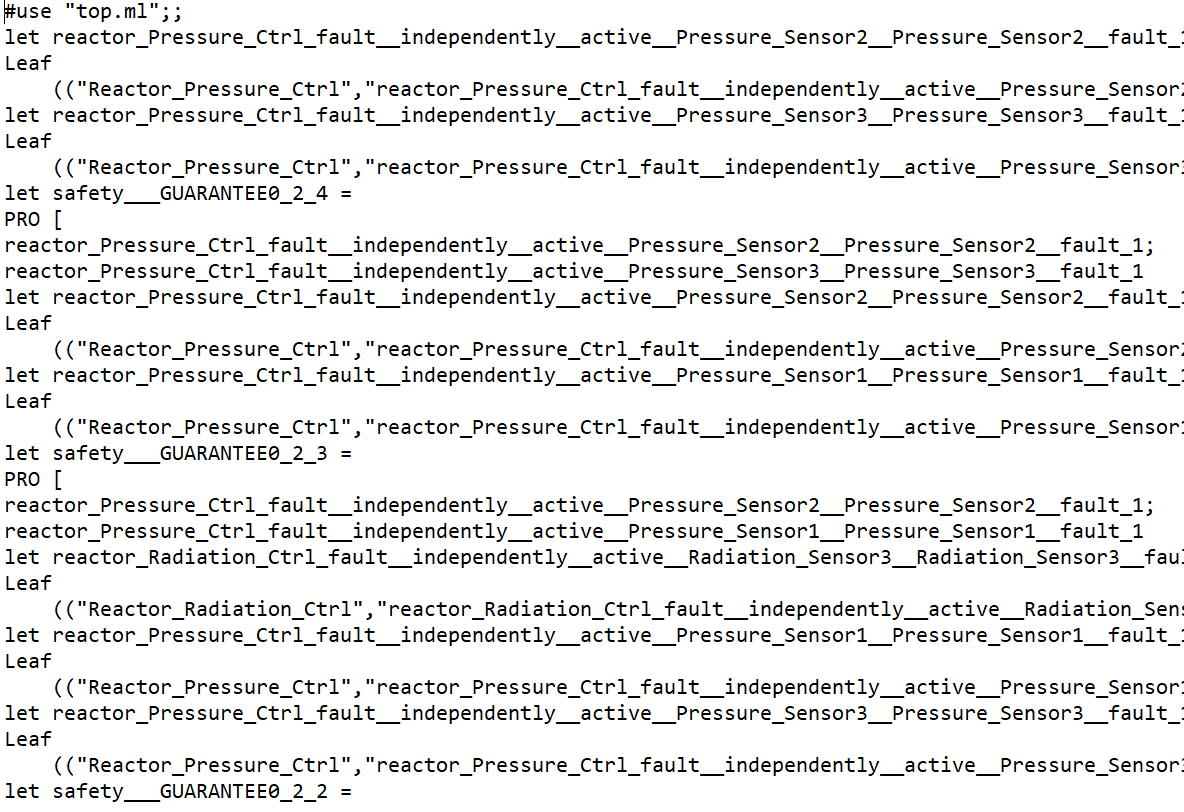
\includegraphics[scale=0.5]{images/soteriaMCS.png}
	\caption{SOTERIA Output of MinCutSets}
		\label{fig:soteriaMCS}
	\end{center}
\end{figure}
\end{comment}

\begin{figure}[htbp]
	%\hspace*{-2cm}
	\vspace{-0.1in} 
	\begin{center}
		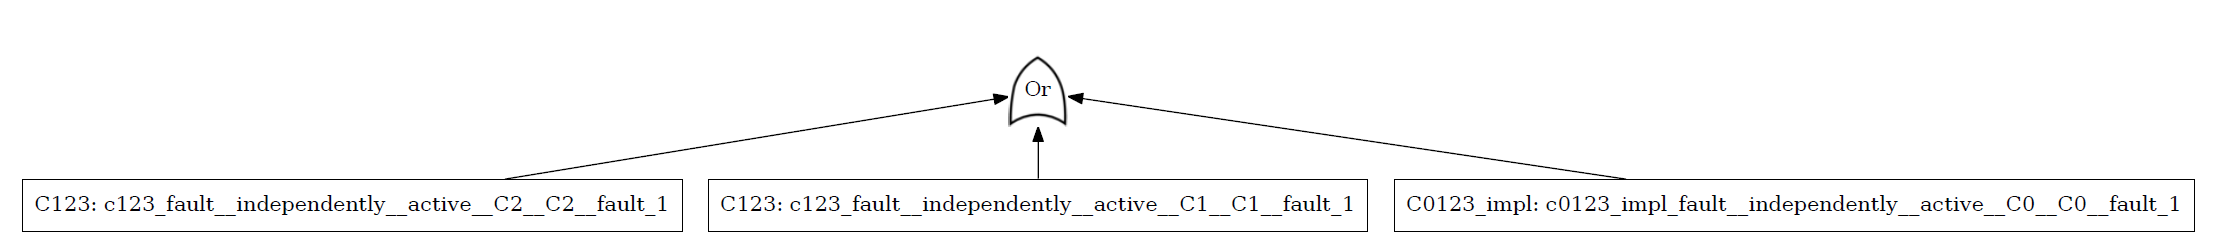
\includegraphics[scale=0.2]{images/Soteria_FT.png}
		\caption{Example SOTERIA Fault Tree}
		\label{fig:soteriaFT}
	\end{center}
%\vspace{-0.5in} 
\end{figure}
\end{enumerate}

\subsubsection{Use of Analysis Results to Drive Design Change}
We use a single top level requirement of the WBS: S18-WBS-0323 (Never indadvertent braking with all wheels locked) to illustrate how Safety Annex can be used to detect design flaws and how faults can affect the behavior of the system). Upon running max $n$ compositional fault analysis with $n = 1$, this particular fault was shown to be a single point of failure for this safety property. A counterexample is shown in Figure \ref{fig:counterexample} showing the active fault on the pedal sensor. 

\begin{figure}[htbp]
	%\vspace{-0.2in}
	\begin{center}
		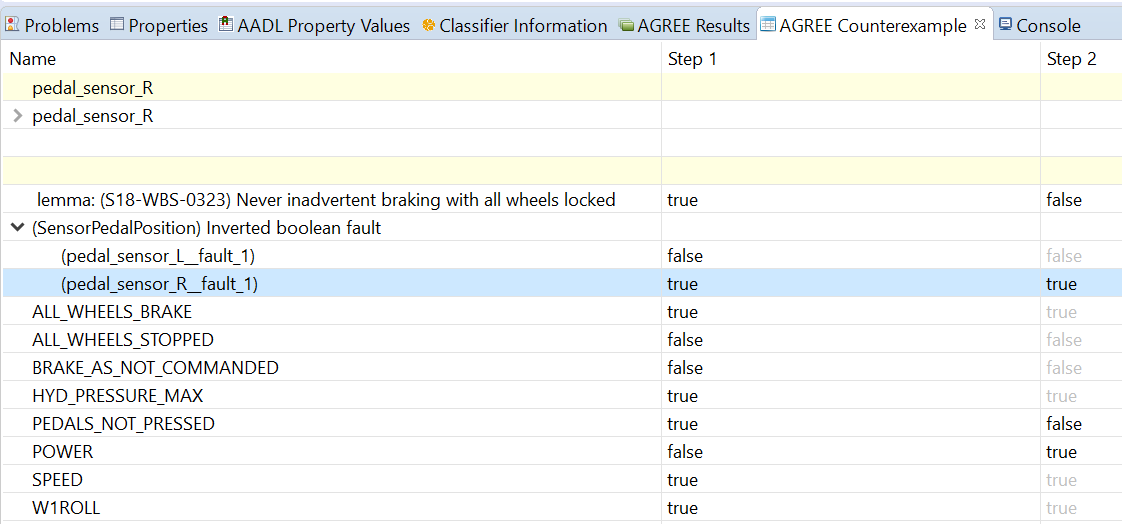
\includegraphics[width=\textwidth]{images/counterexample.png}
	\end{center}
	\vspace{-0.3in}
	\caption{AGREE counterexample for inadvertent braking safety property}
	\label{fig:counterexample}
	%\vspace{-0.2in}
\end{figure} 

Depending on the goals of the system, the architecture currently modeled, and the mitigation strategies that are desired, various strategies are possible to mitigate the problem.

\begin{itemize}
\item Possible mitigation strategy 1: Monitor system can be added for the sensor: A monitor sub-component can be modeled in which it accesses the mechanical pedal as well as the signal from the sensor. If the monitor finds discrepancies between these values, it can send an indication of invalid sensor value to the top level of the system. In terms of the modeling, this would require a change to the behavioral contracts which use the sensor value. This validity would be taken into account through the means of $valid \land pedal\_sensor\_value$. 
%In the real system however, this mitigation would need to be taken into account. Whether this is a flag to the pilot who can then override the electrical system and switch to a different mode or perform some other action to mitigate the failed sensor must be discussed and implemented. 

\item Possible mitigation strategy 2: Redundancy can be added to the sensor: A sensor subsystem can be modeled which contains 3 or more sensors. The overall output from the sensor system may utilize a voting scheme to determine validity of sensor reading. There are multiple voting schemes that are possible, one of which is a majority voting (e.g. one sensor fails, the other two take majority vote and the correct value is passed). 
When three sensors are present, this mitigates the single point of failure problem. New behavioral contracts are added to the sensor system to model the behavior of redundancy and voting. 
\end{itemize}

In the case of the pedal sensor in the WBS, the latter of the two strategies outlined above was implemented. A sensor system was added to the model which held three pedal sensors. The output of this subsystem was constrained using a majority voting scheme. Upon subsequent runs of the analysis (regardless which type of run was used), resilience was confirmed in the system regarding the failure of a single pedal sensor. Figure \ref{fig:sensorsystem} outlines these architectural changes that were made in the model.

\begin{figure}[htbp]
	%\vspace{-0.2in}
	\begin{center}
		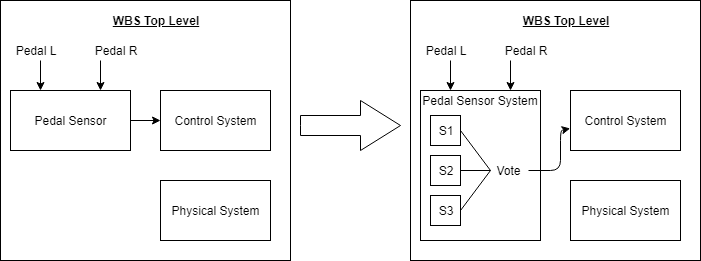
\includegraphics[width=\textwidth]{images/sensorsystem.png}
	\end{center}
	\vspace{-0.3in}
	\caption{Changes in the architectural model for fault mitigation}
	\label{fig:sensorsystem}
	%\vspace{-0.2in}
\end{figure}

As can be seen through this single example, a system as large as the WBS would benefit from many iterations of this process. Furthermore, if the model is changed even slightly on the system development side, it would automatically be seen from the safety analysis perspective and any negative outcomes would be shown upon subsequent analysis runs. This effectively eliminates any miscommunications between the system development and analysis teams and creates a new safeguard regarding model changes. 

For more information on types of fault models that can be created as well as details on analysis results, see the users guide located in the GitHub repository \cite{SAGithub}. This repository also contains all models used in this project. 